\documentclass{article} % For LaTeX2e
\usepackage{nips14submit_e,times}
\usepackage{amsmath}
\usepackage{hyperref}
\usepackage{url}
\usepackage{graphicx}

%\documentstyle[nips14submit_09,times,art10]{article} % For LaTeX 2.09

\title{Reading Minds : Identifying read words using images of brain activity}

\author{
Tomasz Sarkedja \\
Physics Department\\
University of Washington\\
\texttt{tomaszs@uw.edu} \\
\And
Stella Stylianidou \\
Physics Department\\
University of Washington\\
\texttt{stellast@uw.edu} \\
}


\newcommand{\fix}{\marginpar{FIX}}
\newcommand{\new}{\marginpar{NEW}}

\nipsfinalcopy % Uncomment for camera-ready version

\begin{document}


\maketitle

\begin{abstract}
Machine learning techniques are often used to decipher brain images experiments and find whether there are relationships between fMRI data and variables of interest. In this study we show that we can predict the words a participant is reading using the brain activation patterns measured via fMRI, thereby showing that fMRI data contain information about the words read. We are able to predict the relationship between the fMRI's with a set of 218 semantic features. Following that we use the semantic feature scores to guess the words the participant was looking with a success rate of 80\%, which is at the success rate found in literature. 

\end{abstract}

\section{Introduction}

Humans have always sought to understand the brain better. Functional Magnetic Resonance Imaging (fMRI), which is an imaging procedure that measures brain activity by detecting changes associated with blood flow, has been a vital component in medical diagnosis, but also in improving our understanding of the human brain and its biology. The information in an fMRI scan is complicated, dense, and interpreting it requires analysis of complex, multivariate data\cite{Pereira2009S199}. With the advent of machine learning it is now possible to find relationships between fMRI scans and human actions or thoughts that were not possible before, and thus prove that data on brain activation regions contain information about those.

Reading or writing words activates individual neurons in the brain. Data from brain activation recording technologies, fMRI and Magnetoencephalography (MEG), have been shown to be able to predict word meaning \cite{mitchell2008predicting} (Mitchell et al., 2008; Palatucci et al., 2009; Sudre et al., 2012; Murphy et al., 2012b), showing a relationship between word meaning and brain activation. Previous work \cite{mitchell2008predicting} has used 'semantic features', which are properties which are used to characterize the meaning of words. Specifically, each word is represented as point in a higher dimensional space, where each dimension is related to the words meaning such as 'is it an animal?','does it fly?'. Words with similar meaning are expected to have a short distance in the semantic feature space, and the opposite for different meaning. 

In our work we seek to identify machine learning techniques that can be used to identify the word the person was looking at from the fMRI image. Our current model relates each semantic feature separately to the brightness of the voxels. The obtained parameters can then be used to predict the value of each of the semantic features for a given fMRI image. The distance of the words in our dictionary from the predicted semantic features can then be used to predict the word the person was reading. The models will be assessed according to the their word predictive power. Our dataset consists of 60 words, each related to 216 semantic features, which were collected by asking humans to rate each word-semantic feature relationship in a scale of 1-5. Furthermore we have 360 fMRI images from the same subject, 6 for each word, consisting of 20,000 voxels. 



\section{Previous Work}

% something on why semantic features relate to fMRI images and why that's a good thing to use


% and then previous research done on semantic features and fMRI
In \cite{mahtiyarThesis} different (human) subjects were combined in one study.


In \cite{fyshe2014interpretable} they present a new algorithm called JNNSE, that uses semantic features and brain activation data to create a better represantion of semantics. They show that their model is closer to behavioral measurements of semantics more closely, it can be used to predict semantic data of words on which the model was not trained on and it can generalize across technologies and human subjects.  


\section{Methods}
Because fMRI scans are expensive the amount of data one can obtain is limited. This makes training our model difficult because the amount of training data (360) is significantly smaller than the dimensionality of the problem (20,000 voxels). Currently we are using linear regression with L1 regularization (Lasso). We expect a strong reduction in the bias of our trained parameters over non-regularized linear regression. The Lasso is used to predict values of 218 semantic features from our fMRI's. The semantic feature values for the training data are obtained via questionnaire with responses given ratings between 1-5 by the test subject. These data are then centered and normalized.



\subsection{Lasso}

To obtain the parameters that relate the value of a semantic feature to the voxels in the brain images we use linear regression with Lasso. Lasso, as described in Tibshirani (1996) ~\cite{lasso}, constrains the L1 norm, thereby shrinking some weights to exactly zero. This technique therefore obtains sparse solutions, which can be useful in the case that the amount of data is much smaller than the dimensionality of the problem (as in this case), or if we expect that few voxels are related to each word. 

To estimate the weights with Lasso we minimize the following function :

\begin{align*}
w_{Lasso} = argmin \{|| Y - Xw ||^2 + \lambda|w|\}
\end{align*}




\subsection{PCA}

The difficulty with this data set is that our dimensionality is many times higher than the amount of data we have. A possible way to decrease our dimensionality is to use Principal Component Analysis (PCA). Principal Component Analysis transforms a set of observations, which may be correlated, into a a new basis where the set of values are linearly uncorrelated. The new basis for the data is chosen in a way such that the components are in order of accounting for the largest possible variance in the data. 


\subsection{Non linear features}



\section{Results}


\subsection{Obtaining the best lambda}
In order to choose a $\lambda$ suitable for our dataset we used pathwise optimization ~\cite{friedman2010regularization}. In pathwise optimization we start with a high value for  $\lambda$ and solve the optimization for a decreasing series of lambdas using the previous results for our weights. We finally choose the $\lambda$ with the smallest root mean square error on a validation set, which is a subset partitioned from our training data. Since the semantic features consist of similar relationships, we attempted to choose the best $\lambda$ for our dataset using one of the semantic features. 250 fMRI images were used to train our dataset and 50 were used as validation data. We started from maximum lambda calculated as $2 * max (|X^T.(y - <y>)|)$ and decreased the $\lambda$ by multiplying by 0.8 in each iteration. Choosing the lambda using this method on different semantic features obtained similar values for all features, but larger values than expected (~134). In figure 1, we shown the root mean square error on the training data and validation data versus different $\lambda$. This large value of $\lambda$ creates a very sparse solution and sets most of the features to 0. The reason behind the large value of lambda may be due to the nature of the data, or the large dimensionality compared to the amount of training data we have.



\begin{figure}[h]
\begin{center}
%\framebox[4.0in]{$\;$}
%\fbox{\rule[-.5cm]{0cm}{4cm} \rule[-.5cm]{4cm}{0cm}}
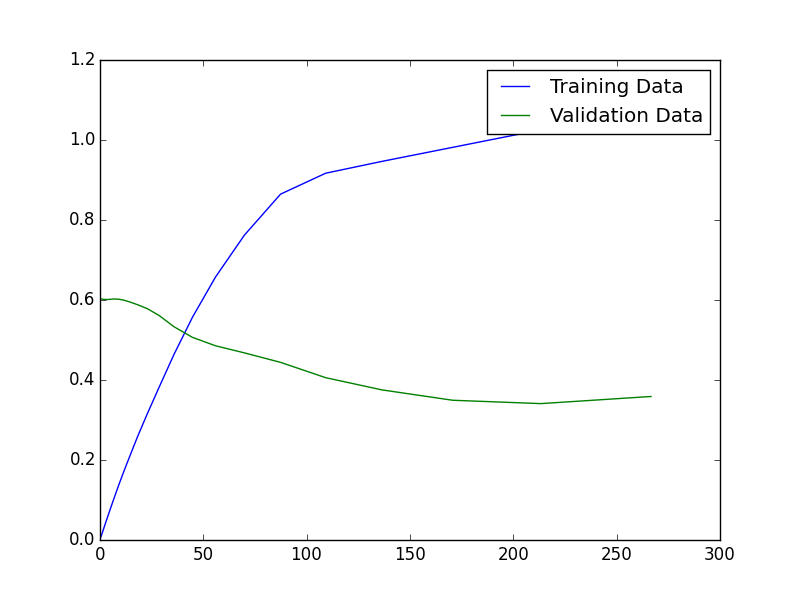
\includegraphics[scale=0.5]{trainvalidlambda.png}
\end{center}
\caption{Training lambdas on the first semantic feature on 250 data, and using 50 fMRI
images as a validation test. Horizontal axis: value of lambda. Vertical axis: RMSE. The data suggest strong overfitting on our training set.}
\end{figure}

Following this initial test we tried cross validating our choice of $\lambda$. For each step we chose 60 fMRIs to be our validation set and then used the remaining 240 fMRI's as our training set. We still used holdout set of 60 for testing. The results were largely indistinguishable from performing single step validation, except that one of the $\lambda$ returned was much smaller than the rest. This discrepancy suggests that our current method of choosing a lambda is ill informed, probably due to the homogeneity of our semantic feature data. Currently we believe that it may be necessary to choose a $\lambda$ based on several semantic features, because doing so would resolve the problem of the homogeneity of the semantic features.





\subsection{Results on the test data}


\subsection{Predict out of two}
Our goal was to be able to predict out of two words the word that the subject was looking at during the time the fMRI image was taken. The predicted semantic feature values were compared to the semantic features of the two given words and the word for which the semantic features have the smallest distance from the predicted semantic features was chosen. Our accuracy was measured as the percentage of correctly predicted words out of the two choices. 

Our first attempt was to use lasso. We used different methods of cross validation, to obtain the best $\lambda$  that had the lowest RMSE on the validation set and then train lasso on the data. Using this method our results were close to random with only 52\% of the words guessed correctly (31 out of 60), indicating that the weights predicted are not satisfactory for the prediction of the semantic features. The root mean square error on our training data set was \~0.25, where as on our test data set it was of the order of 22000. 

The poor results, possibly due to the high dimensionality of our data, led us to consider PCA to decrease the dimensions. Using PCA with 300 principal components and then using linear regression with Lasso to train our model we obtained 70\% accuracy, which is higher than random. 



\subsection{Word Ranking}


\section{Discussion}


\subsection{Semantic Features}

In our study we used 216 semantic features to predict a single word. A question that we could ask is whether using all those semantic features improves the accuracy of our study. The first figure shows that indeed that the use of more semantic features improves our accuracy, with a very steep increase in accuracy with the addition of the first 20 semantic features, and then a slow increase up to about the 120th semantic feature at which point the accuracy fluctuates between 0.75  - 0.8. In order thus to capture as much of the meaning of the word as possible, many semantic features are needed.

\begin{figure}[h]
\begin{center}
%\framebox[4.0in]{$\;$}
%\fbox{\rule[-.5cm]{0cm}{4cm} \rule[-.5cm]{4cm}{0cm}}
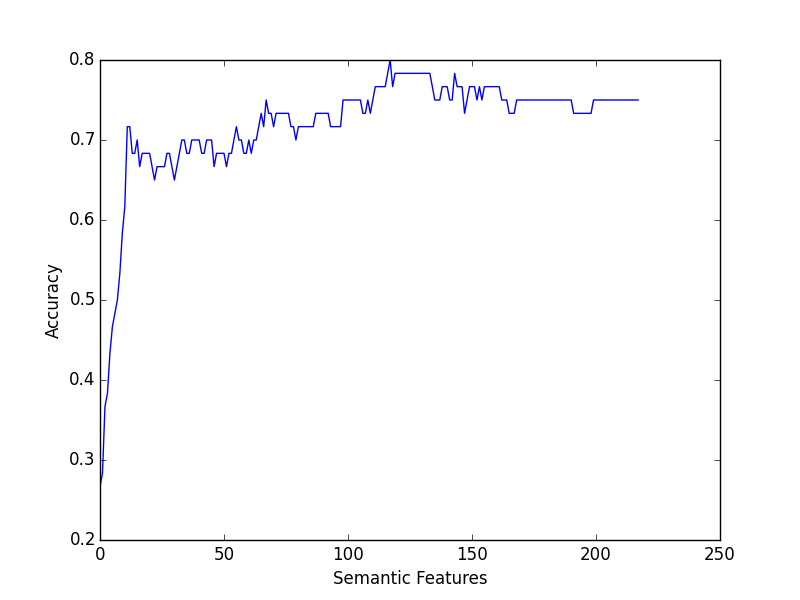
\includegraphics[scale=0.5]{accuracyVSnumFeatures.png}
\end{center}
\caption{Accuracy versus number of features used}
\end{figure}

A second question we may ask is whether one semantic feature outperforms or under-performs the others. In the figure below we have

\begin{figure}[u]
\begin{center}
%\framebox[4.0in]{$\;$}
%\fbox{\rule[-.5cm]{0cm}{4cm} \rule[-.5cm]{4cm}{0cm}}
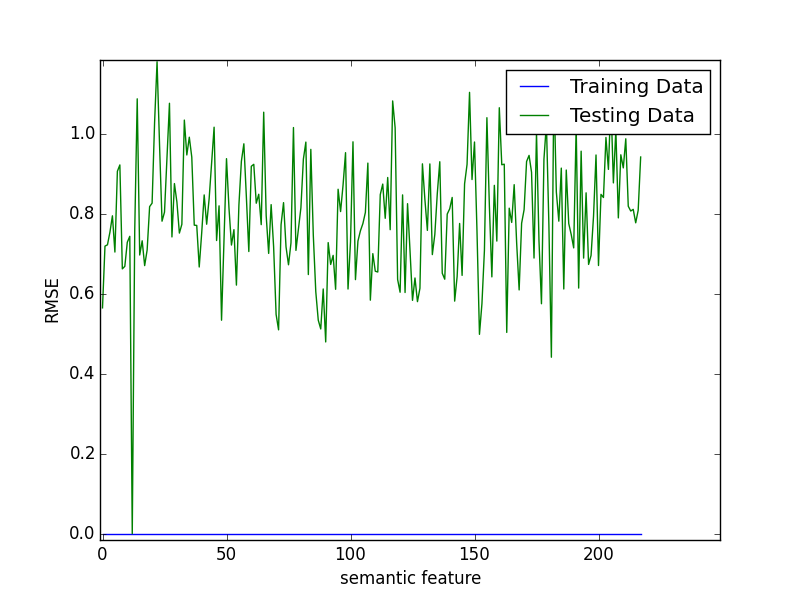
\includegraphics[scale=0.5]{rmse_train_test.png}
\end{center}
\caption{Root mean square error for each semantic feature on training and test data.}
\end{figure}






\subsection{Mistakes}


\begin{figure}[h]
\begin{center}
%\framebox[4.0in]{$\;$}
%\fbox{\rule[-.5cm]{0cm}{4cm} \rule[-.5cm]{4cm}{0cm}}
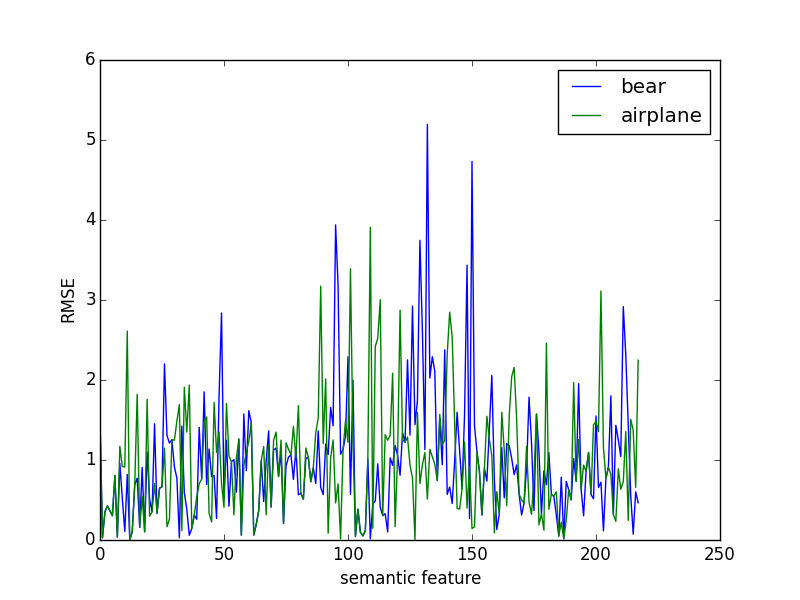
\includegraphics[scale=0.5]{mistaken_word0.png}
\end{center}
\caption{RMSE with pca dimensions}
\end{figure}

\begin{figure}[h]
\begin{center}
%\framebox[4.0in]{$\;$}
%\fbox{\rule[-.5cm]{0cm}{4cm} \rule[-.5cm]{4cm}{0cm}}
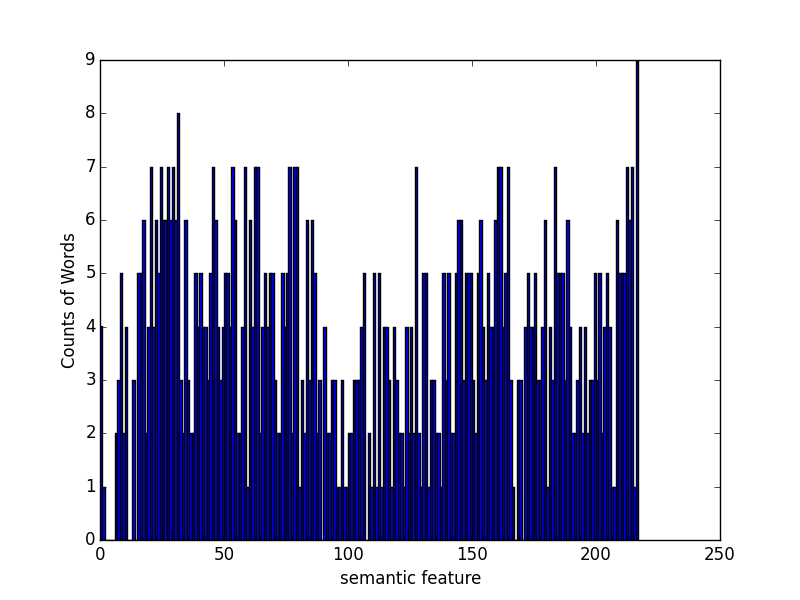
\includegraphics[scale=0.5]{rmse_correct_incorrect_per_semantic_Feature.png}
\end{center}
\caption{RMSE with pca dimensions}
\end{figure}



\subsection{Predicting words outside the dataset}


\subsection{Analysis on the PCA dimensions}


\begin{figure}[h]
\begin{center}
%\framebox[4.0in]{$\;$}
%\fbox{\rule[-.5cm]{0cm}{4cm} \rule[-.5cm]{4cm}{0cm}}
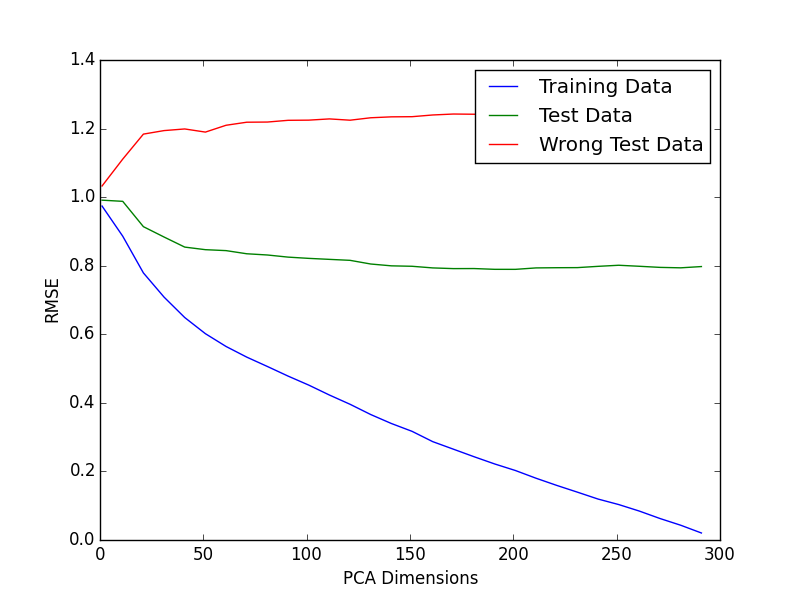
\includegraphics[scale=0.5]{rmse_with_pca_dimensions.png}
\end{center}
\caption{RMSE with pca dimensions}
\end{figure}


\begin{figure}[h]
\begin{center}
%\framebox[4.0in]{$\;$}
%\fbox{\rule[-.5cm]{0cm}{4cm} \rule[-.5cm]{4cm}{0cm}}
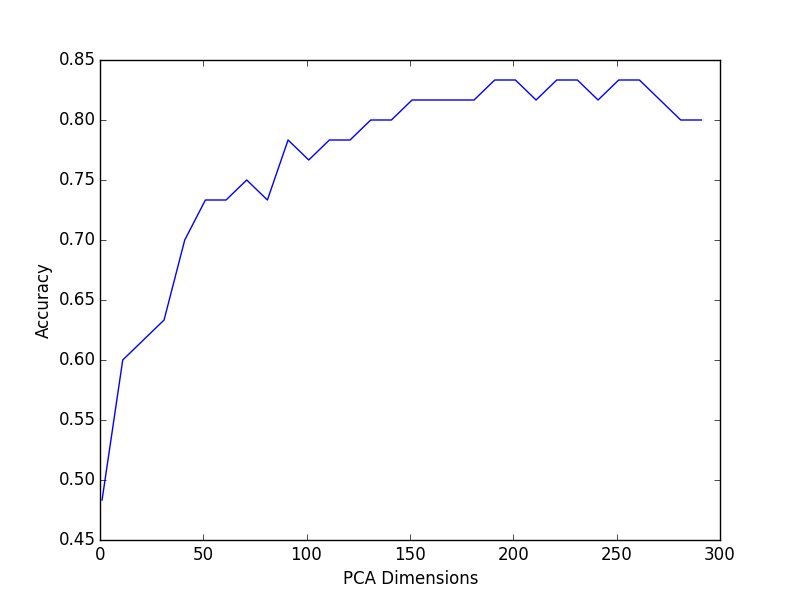
\includegraphics[scale=0.5]{accuracy_2of2.png}
\end{center}
\caption{RMSE with pca dimensions}
\end{figure}




\subsection{Comparison of our method with previous work}
I am a choo choo train!!!


\bibliographystyle{unsrt}
\bibliography{referencesfMRI}

\end{document}
